\chapter{Data acquisition and annotation \status{in progress}}
	\label{chap:data}
	
	This chapter describes the data that influenced the decisions of selecting the cell detection and tracking methods. In \cref{sec:data_examples} we briefly describe the imaging method used to acquire the image sequences and present some example datasets. \Cref{sec:data_tool} presents the data annotation tool that was developed to ease the data annotation process and in \cref{sec:data_annotation} we discuss how the tools was used for annotating the datasets, and the difficulties that were encountered.

    \section{Data acquisition and example datasets \status{in progress}}
    \label{sec:data_examples}
    
    As discussed in the concluding section of \cref{chap:relatedwork} the datasets heavily influence the choice of algorithms for cell detection and tracking. Many computer vision algorithms rely on heuristics to improve their accuracy. In cell detection methods, this is obvious from the fact that a method developed for a certain type of imaging method will likely perform poorly on an image sequence of different types of cells (e.g. different shape of cells). In cell tracking heuristics help adjust the algorithms to the specific behaviour of cells that are being analysed. For example, a different tracking method could be used for images with cells that move slowly (and there is a large overlap between cells in consecutive frames) than for cells that move quickly (and there is little overlap between cells in consecutive frames).
    
    The data acquisition process is not part of this research. However, for the reasons stated above, it is important to understand how the images were obtained and know the characteristics of the datasets. Below, we outline the image acquisition process, and then present some of the datasets we wish to analyse.
    
    The image sequences that inspired the development of the methods describe in this thesis were acquired \textit{in vivo}. This means that the images are obtained on living mice, in contrast to \textit{in vitro} where cells are analysed on a tissue sample in a standard laboratory environment using petri dishes and other instruments. \textit{In vivo} analysis is preferred over \textit{in vitro} because it is better suited for observing the behaviour of cells in their natural environment.
    
    \todo[inline]{Ask Leo: Info about the ventilator method. Is it two-photon mocroscopy? What camera was used to capture the images?}
    
    \todo[inline]{Extract from the paper Leo gave me: More recently, the introduction of microscopes allowering for thicher tissue penetraction and higher resolution (spinning-disc and two-photon microscopes), more complex tissuea dn organs, sucha as the skin, lives, brain and lung, can also be imaged. The observation of the lung was a challenge for a long time owing to motion artefacts. 
        
    The introbutio of fluorescence (confocal) microscopy  in combination with spinning-disc and two-photon microscopes  has allowed the use of fluorescent antibodies for labelling different cell populations on anatomical structures, as well as the use of transeenic mice with fluorescent leukocyte subsets. }
    
    All the data was provided by Dr. Leo Carlin from the Leukocyte Biology Section at the National Heart and Lung Institute (NHLI)\footnote{\url{http://www1.imperial.ac.uk/nhli/}}.
    
    \subsection{Datasets \statusfirstdraft}
       
	From the datasets provided by Dr. Leo Carlin, five have been selected to use in the evaluation of this work because of their distinct characteristics. The original dimensions of the datasets were 512-by-512 pixels, but some have been cropped to reduce the number of cells to annotate.
	
	\todo{Use the detector to compute the average number of cells in each dataset}

	\subsubsection{Dataset A}
	\todo[inline]{This is series30green}
	\begin{figure}[h]
   		\begin{subfigure}{.32\textwidth}
   		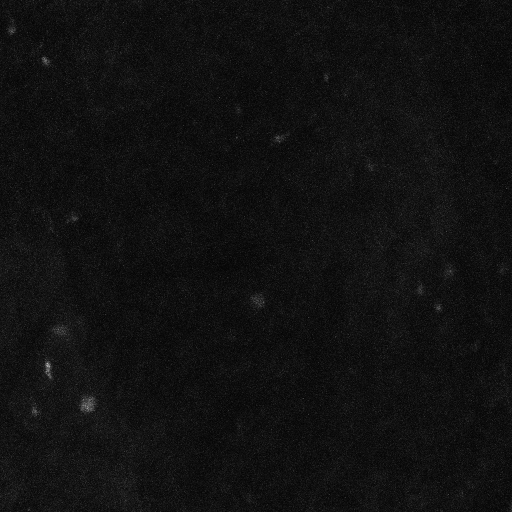
\includegraphics[width=\textwidth]{images/series30green019}
   		\end{subfigure}%
   		\hfill
   		\begin{subfigure}{.32\textwidth}
   		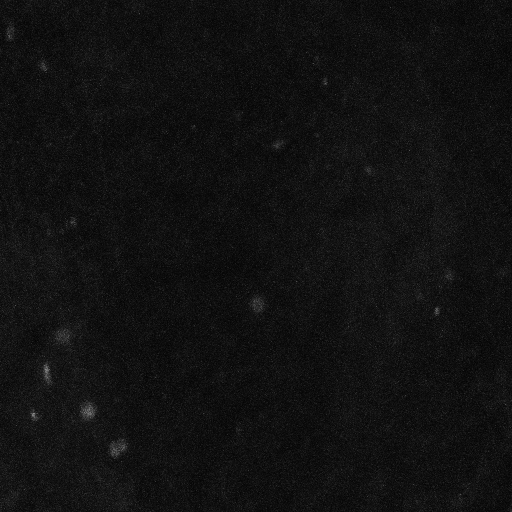
\includegraphics[width=\textwidth]{images/series30green020}
   		\end{subfigure}
   		\hfill
   		\begin{subfigure}{.32\textwidth}
   		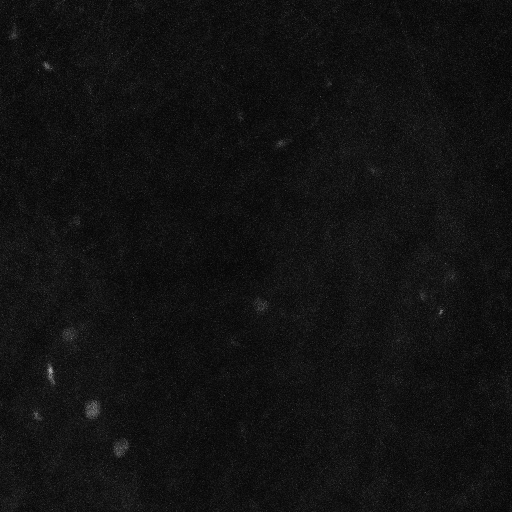
\includegraphics[width=\textwidth]{images/series30green021}
   		\end{subfigure}
   		\caption{Three consecutive frames from dataset A.}
   		\label{fig:data_datasetA}
   	\end{figure}
   	
   	This is a dataset obtained from the lung\todo{Lung for sure?}. This dataset contains a very low cell density (about 3 cells per frame). The image sequence contains 66 frames, all of which were annotated. The cells appear grey on a dark, relatively homogeneous, background. The cell boundaries smoothly blend into the background. The images are of constant quality, and there are few significant camera artefacts. The cells move slowly. The dimensions of the images is 512-by-512 pixels.
   	
   	\todo[inline]{What is the difference between these cells and the ones in dataset B? They are taken simultaneously... on is series30red the other series30green}
   	
	\subsubsection{Dataset B}
	\todo[inline]{This is series30red}
	\begin{figure}[h]
		\begin{subfigure}{.32\textwidth}
		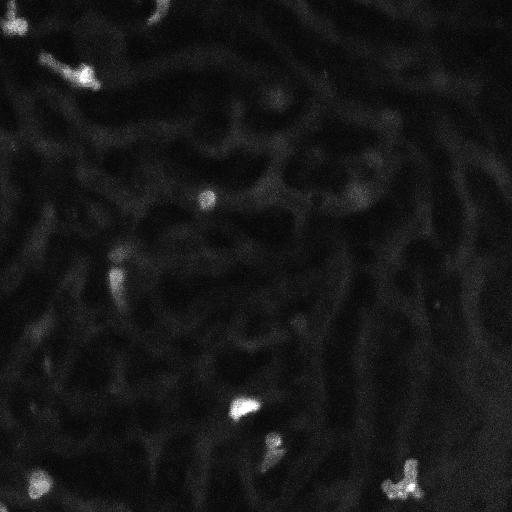
\includegraphics[width=\textwidth]{images/series30red024}
		\end{subfigure}%
		\hfill
		\begin{subfigure}{.32\textwidth}
		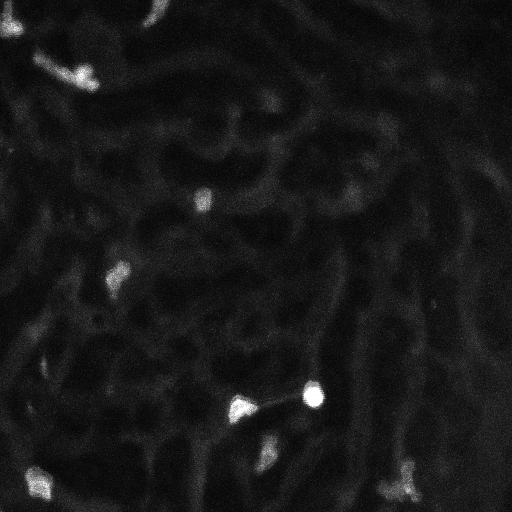
\includegraphics[width=\textwidth]{images/series30red025}
		\end{subfigure}
		\hfill
		\begin{subfigure}{.32\textwidth}
		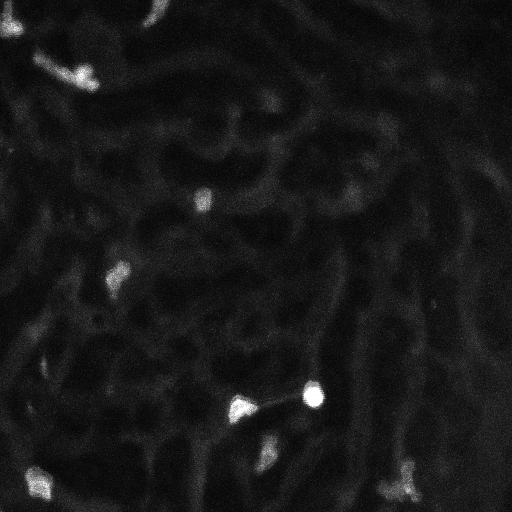
\includegraphics[width=\textwidth]{images/series30red025}
		\end{subfigure}
		\caption{Three consecutive frames from dataset B.}
		\label{fig:data_datasetB}
	\end{figure}
	
	This dataset is also obtained from the lung\todo{Lung for sure?}. In fact, it was obtained simultaneously with dataset A, but represents a different types of cells \todo{Ask Leo to help me specify}.The cells appear brighter than in dataset A, but their shapes vary. Some are round and others elongated and deformed to fit into the tight blood vessels \todo{Are thes blood vessels?} in which they move. In the background we can clearly discern the blood vessels in a darker grey colour. Cells in this dataset are more active in movement. The images are of constant quality, and there are few significant camera artefacts. The dataset contains 66 frames, of which all have been annotated. The dimensions of the images is 512-by-512 pixels.
		
	\subsubsection{Dataset C}
	\todo[inline]{This is series13green}
    \begin{figure}[h]
    	\begin{subfigure}{.32\textwidth}
    		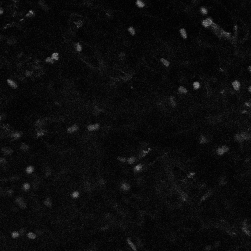
\includegraphics[width=\textwidth]{images/series13greencropped008}
    	\end{subfigure}
    	\hfill
    	\begin{subfigure}{.32\textwidth}
	    	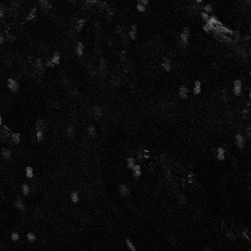
\includegraphics[width=\textwidth]{images/series13greencropped009}
    	\end{subfigure}
   		\hfill
  	    \begin{subfigure}{.32\textwidth}
   	  		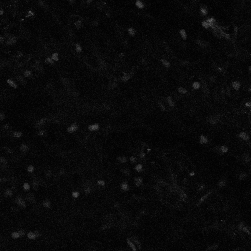
\includegraphics[width=\textwidth]{images/series13greencropped010}
  	    \end{subfigure}
    	\caption{Three consecutive frames from dataset C.}
    	\label{fig:data_datasetC}
    \end{figure}
    
    This dataset is also obtained from the lung\todo{Lung for sure?}. The range of brightness of the cells is large. Some are clearly visible, some barely stand out of the background. Their shape is relatively consistent. The background is dark, with some very faint cells. The cells are stagnant in their position on the tissue, but the lung tissue is moving due to the breathing of the mice. For this reason, the dataset contains many motion artefacts. Some frames are blurred, and many appear to contain the same copies of the cells slightly shifted, as seen in the second image in \cref{fig:data_datasetC}. The cell density is very high in this dataset (about 40 cells per frame). The dataset consists of 126 frames, of which 55 were manually annotated. The dimensions of the cropped images is 251-by-251 pixels.

	\subsubsection{Dataset D}
	\todo[inline]{This is series14croppedclean}
	\begin{figure}[h]
		\begin{subfigure}{.32\textwidth}
		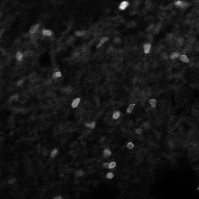
\includegraphics[width=\textwidth]{images/series14croppedclean024}
		\end{subfigure}%
		\hfill
		\begin{subfigure}{.32\textwidth}
		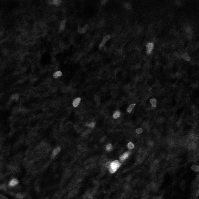
\includegraphics[width=\textwidth]{images/series14croppedclean025}
		\end{subfigure}
		\hfill
		\begin{subfigure}{.32\textwidth}
		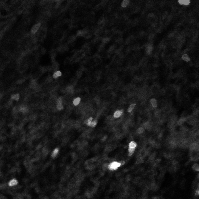
\includegraphics[width=\textwidth]{images/series14croppedclean027}
		\end{subfigure}
		\caption{Three consecutive frames from dataset D.}
		\label{fig:data_datasetD}
	\end{figure}

	Dataset D is obtained from the liver \todo{Liver for sure?}. The cells are well discernible from the background, which can contain some very faint cells. The cell boundaries are clearly visible. The cell density is about 12 cells per frame. The original dataset contained 682 frames. Unfortunately, the dataset contained large sequences of frames that were of exceedingly low quality, such that even a human could not track the cells in the dataset. Thus, the dataset has been pruned to 377 frames of dimensions 199-by-199 pixels. The dataset contains many motion artefacts, the contrast is constantly changing, and often about half of the cells in each frame become invisible for a few frames, even after manually eliminating the worse frames.
	
	\subsubsection{Dataset E}
	\todo[inline]{This is seriesm170\_13cropped}
	\begin{figure}[h]
	
		\begin{subfigure}{.32\textwidth}
		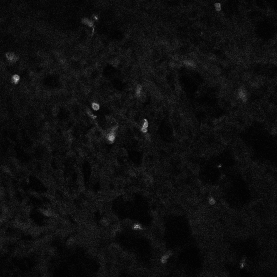
\includegraphics[width=\textwidth]{images/seriesm170_13cropped016}
		\end{subfigure}%
		\hfill
		\begin{subfigure}{.32\textwidth}
		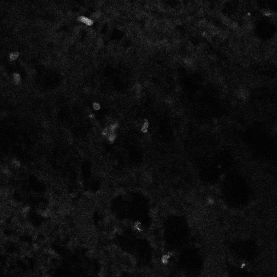
\includegraphics[width=\textwidth]{images/seriesm170_13cropped017}
		\end{subfigure}
		\hfill
		\begin{subfigure}{.32\textwidth}
		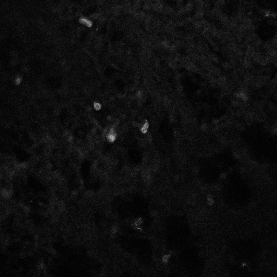
\includegraphics[width=\textwidth]{images/seriesm170_13cropped018}
		\end{subfigure}
		\caption{Three consecutive frames from dataset E.}
		\label{fig:data_datasetE}
	\end{figure}
    
    \todo{Where is the dataset from?}The cells in this dataset are smaller. Some appear bright, while others darker, which makes them sometimes difficult to recognize from the dark background. The density of the bright cells is about 8 per frame of dimensions 277-by-277 pixels. For the purpose of analysing their behaviour we are only interested in these bright cells. The sequence contains 194 frames, of which 65 have been manually annotated. The images become darker in the later parts of the image sequence. The background is stable, but there is an alternating dark/bright area probably caused by the camera shutter.
    	
	\subsection{Imaging analysis challenges \statusnew}
	
	In this section we are going to present two phenomena caused by moving tissue and the camera shutter that make this datasets especially hard to track for frame-by-frame tracking methods.
	
	The first challenge is the artefacts caused by the camera shutter. These appear as alternating dark/bright horizontal patches which seem to move from the top to the bottom of the images. The effect can be seen in \cref{fig:data_challenge_shutter}. This makes the tracking problem difficult, because the cells behind the dark areas appear fainter or disappear completely for the few frames that they are covered.
		
	\begin{figure}[h]
	
		\begin{subfigure}{.32\textwidth}
		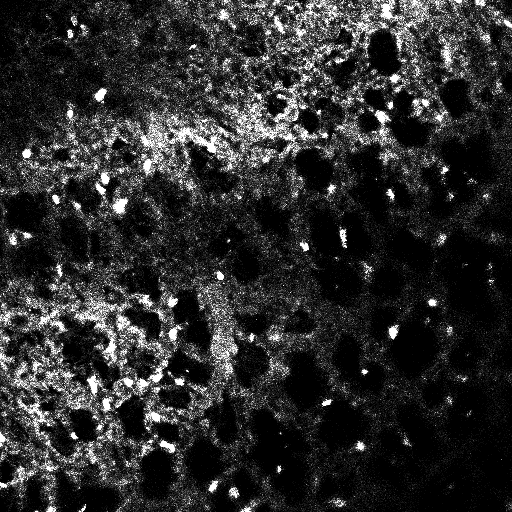
\includegraphics[width=\textwidth]{images/shutterseriesm170_13cropped001}
		\end{subfigure}%
		\hfill
		\begin{subfigure}{.32\textwidth}
		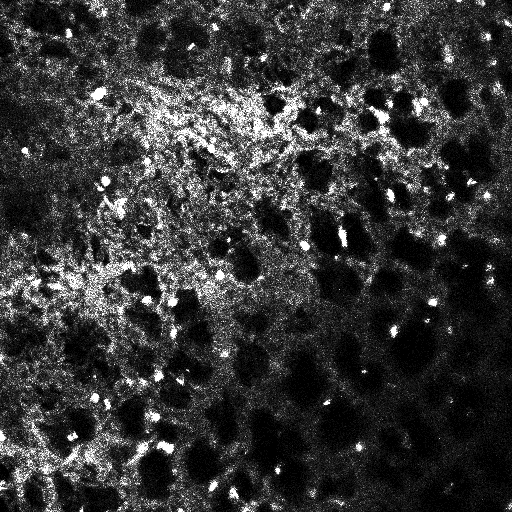
\includegraphics[width=\textwidth]{images/shutterseriesm170_13cropped002}
		\end{subfigure}%
		\hfill
		\begin{subfigure}{.32\textwidth}
		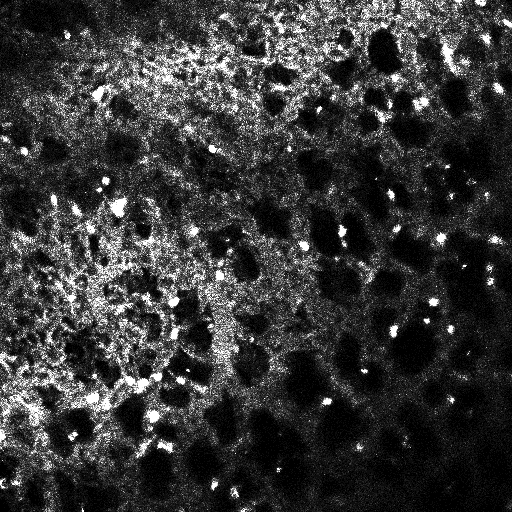
\includegraphics[width=\textwidth]{images/shutterseriesm170_13cropped003}
		\end{subfigure}%
		\vspace{0.2cm}
		\begin{subfigure}{.32\textwidth}
		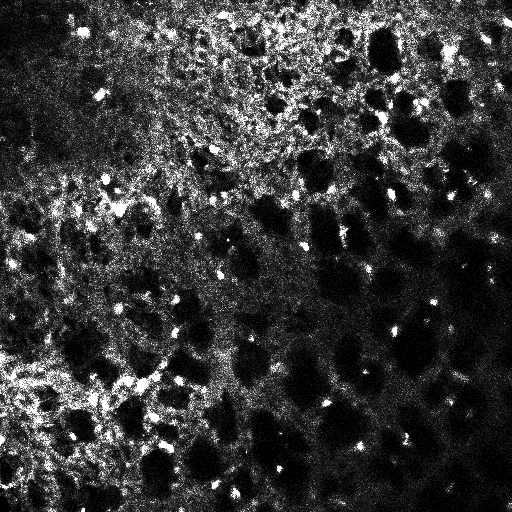
\includegraphics[width=\textwidth]{images/shutterseriesm170_13cropped004}
		\end{subfigure}%
		\hfill
		\begin{subfigure}{.32\textwidth}
		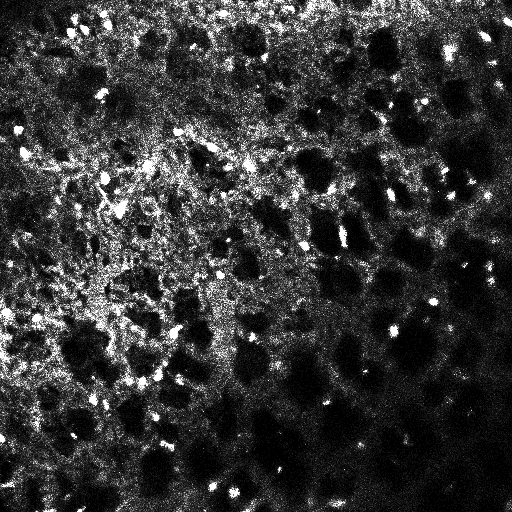
\includegraphics[width=\textwidth]{images/shutterseriesm170_13cropped005}
		\end{subfigure}%
		\hfill
		\begin{subfigure}{.32\textwidth}
		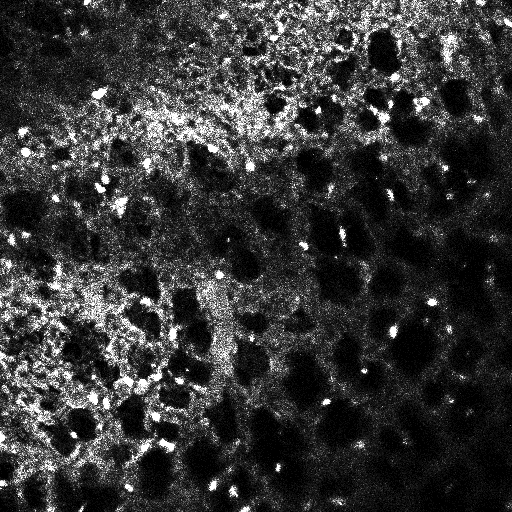
\includegraphics[width=\textwidth]{images/shutterseriesm170_13cropped006}
		\end{subfigure}
		\caption{Six consecutive frames from a sequence displaying the alternating dark/bright regions caused by the camera shutter. The contrast and sharpness of the images has been edited to dramatize the effect.}
		\label{fig:data_challenge_shutter}
	\end{figure}
	
	The second challenge is the movement of the tissue, especially in the case of lung imaging. The fast breathing pace of mice causes a sensation that the image is shaking. The shaking can be in the x-y plane, but sometimes, as in the case shown in figure \cref{fig:data_challenges_movement} it can be primarily in the z-direction. Displacement in the x-y direction causes the cells to jiggle. Displacement of the tissue in the z-direction causes part of all of the image to become out-of-focus for a few frames.
	
	\begin{figure}[h]

		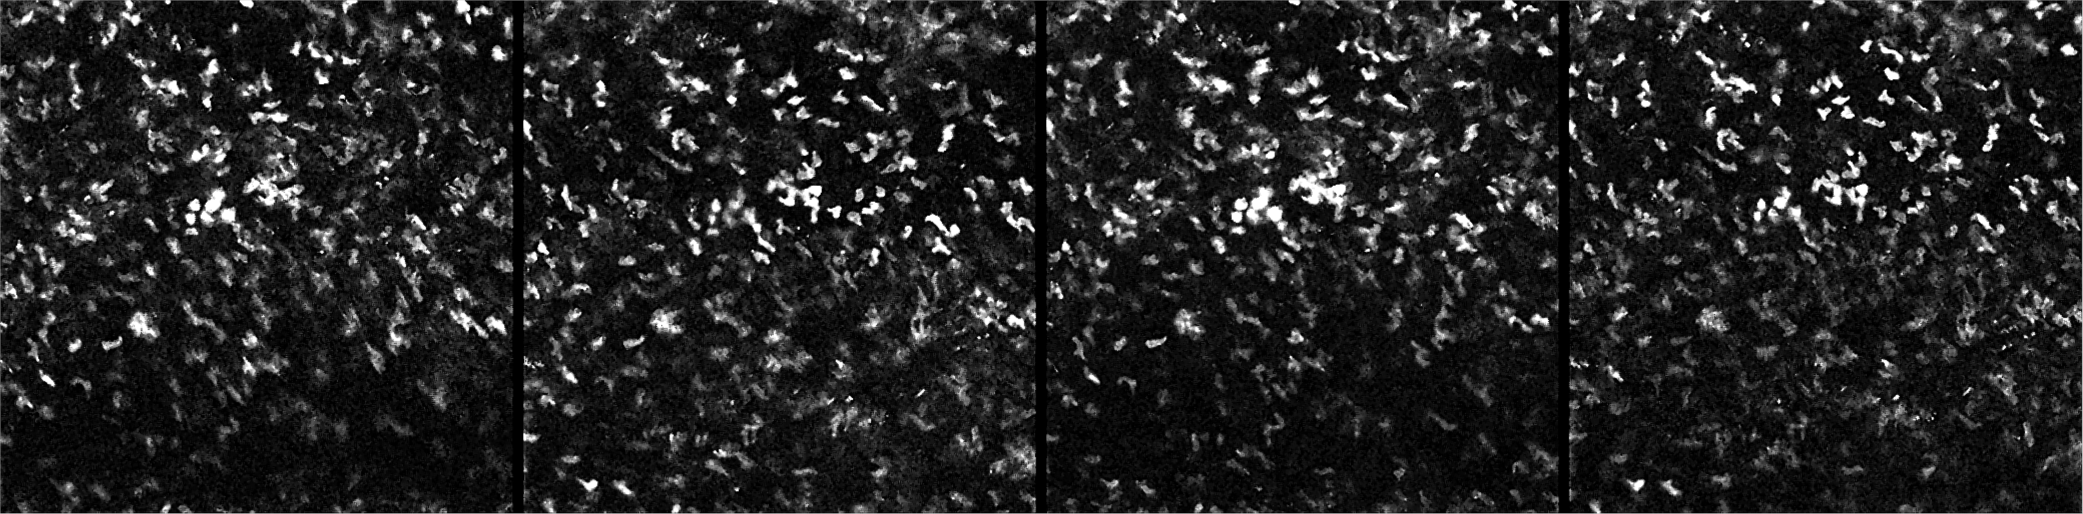
\includegraphics[width=\textwidth]{images/data_challenge_movement}

		\caption{Four consecutive frames taken from the lung displaying varying cell clarity due to the displacement caused by the lung movement.}
		\label{fig:data_challenges_movement}
	\end{figure}
	
	Several of the datasets present these phenomena to a lesser or larger extend. These artefacts where the primary reason for choosing a global optimization method for associating detection responses into trajectories.

    \todo{Write what parameters were used for the tracker}
    \section{The annotation tool \statusnew}
    \label{sec:data_tool}
    
    	\todo[inline]{some notes on the importance of accurate annotation,s advantages and disadvantages of dot annotations.}
    
    	\todo[inline]{Describe the requirements of an efficient cell annotation tool, such as multipreview, linking, zooming, correct interpretation and saving of the dataformat}
    	
    	\todo[inline]{An overview of the annotation GUI}
    	the multiple displays
    	filter
    	tools for additing/deleting dots and links
    	simultaneous display of detections and links    
    	
    	\todo{The feature of the tool}
    
    	\todo{A user guide is provided in the appending}
    \section{Annotating cell images \status{new}}
    \label{sec:data_annotation}
    
    \todo{Briefly explain who made the annotation}
    \todo{Explain who reviewed them}
    \todo{Explain how good the annoations are}
    \todo{Explain if more detailed annotation would result in better results}
    \rewrite{This describes annotation using Fiji, which was only used at the beginnig}
    What follows is a description of the process of image annotation for use in the machine learning algorithm to detect cells. The image annotation, as required by Arteta's \cite{arteta12} algorithm, are dots on each cell of the image. The algorithm uses these dots as positive examples, and all the remaining pixels as negative examples of a cell.
    
    We have annotated a subset of frames on the Lung dataset provided by Dr. Leo Carlin. The entire dataset is composed of 150 frames, and is divided into two channels, one for each type of cell (\todo{I need to learn more about the types of cells I am tracking}). We have marked 10 cropped frames on each channel (frame 1, 14, 25, 46, 81, 115, 131, 143 and 150) of dimensions about $128\times118$ pixels.
    
    The annotation was performed using a Fiji \cite{fiji12} tool called PointPicker \cite{thevanez14} which is accessible from \(Analyse/Tools/PointPicker\). The annotation is done by manually clicking on each identified cell.The tool outputs a $txt$ file containing $x$ and $y$ coordinates of each annotation, the image number, as well as some other metadata that is not important for us.
    
    \begin{figure}
    	\begin{subfigure}{.49\textwidth}
    	  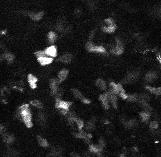
\includegraphics[width=\textwidth]{images/seq_red_crop}
    	\end{subfigure}%
    	\hfill
    	\begin{subfigure}{.49\textwidth}
    	  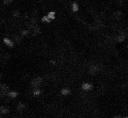
\includegraphics[width=\textwidth]{images/seq_green_crop}
    	\end{subfigure}
    	\caption{Examples of a cropped frame that was annotated for the cell detection machine learning algorithm. Each frame belongs to a different channel of the dataset.}
        \label{fig:annotation_image}
    \end{figure}
    
    It must be noted that the images are very noisy, and it is often hard to distinguish cells from non cells. Figure \ref{fig:annotation_image} displays an example of an image that was annotated. It is therefore questionable how accurately the learning method will be able to learn the idea of a cell, given that the annotations are far from perfect. It would have been much easier to perform the learning using a synthetic dataset.
    
    The data is then loaded into MATLAB and converted into the format required by the algorithm. The data tidying is performed by the script \textit{prepareTrainData.m}.